% ===========================================
Denote by $\mathfrak{S}$ the class of all numerical semigroups. Let $\mathfrak{W}=\{S\in\mathfrak{S}\mid \wilfoper(S)\ge 0\}$ and let $\mathfrak{E}=\{S\in\mathfrak{S}\mid \eliahouoper(S)\ge 0\}$. 

Whether $\mathfrak{S}=\mathfrak{W}$ is presently not known (Wilf's conjecture says that the equality holds, but it is still a conjecture).
That $\mathfrak{E}\subseteq \mathfrak{W}$ follows from Proposition~\ref{prop:eliahou-implies-wilf}, and up to genus $60$ there are exactly $5$ numerical semigroups not in $\mathfrak{E}$, thus showing that the inclusion is strict (the examples were obtained by Fromentin and appear in~\cite[pgs~2112,2113]{Eliahou2018JEMS-Wilfs}).
%
The following is a consequence of Remark~\ref{rem:non-eliahou}.
\begin{fact}\label{fact:infinite-non-eliahou}
	$\mathfrak{W}\setminus \mathfrak{E}$ is infinite.
\end{fact}

Let $\mathcal{P}$ be a property (about numerical semigroups). For instance, ``$\embeddingdimensionoper\ge 3$'' is such a property.
Let $\mathfrak{P}=\{S\in\mathfrak{S}\mid S\models \mathcal{P}\}$ be the class of numerical semigroups satisfying $\mathcal{P}$. With this notation, most results in the previous sections can be written in the following form: ``If $S\in\mathfrak{P}$, then $S\in \mathfrak{W}$.'', or ``If $S$ satisfies $\mathcal{P}$, then $S$ is Wilf''. 

I invite the reader to think an all the results as if they had been written in this form. Some properties cannot be as nicely written as in the above example (``$\embeddingdimensionoper\ge 3$''). However, for instance, the statement ``We say that $S$ satisfies property $\mathcal{P}$ if and only if $S$ is of the form $S(p)$, with $p$ an even positive integer.'' allows to write Proposition~\ref{prop:S(q)} in the above form.

By doing so, one can associate a property to each result and conversely. 
Although I do not intend to explicitly give names to all the properties corresponding to the results stated, there are some exceptions:
\begin{itemize}[leftmargin=*]
	\item[]$\mathbf{\mathcal{D}_3}$ stands for the property ``$\embeddingdimensionoper\ge 3$'', which is associated to Theorem~\ref{th:type<=3}. The corresponding class of semigroups is $\mathfrak{D}_3$. 
\end{itemize} 
	Similarly, one has the correspondences:
\begin{itemize}[noitemsep,leftmargin=*]
	\item[]$\mathbf{\mathcal{D}}$ --- ``$3\embeddingdimensionoper\ge \multiplicityoper$'' --- Theorem~\ref{th:large-embedding-dim-3} --- $\mathfrak{D}$;
	\item[]$\mathbf{\mathcal{M}}$ --- ``$\conductoroper\le 3\multiplicityoper$'' --- Theorem~\ref{th:large-mult-Wilf-jems} --- $\mathfrak{M}$;
	\item[]$\mathbf{\mathcal{G}_{60}}$ --- ``$\genusoper \le 60$'' --- Theorem~\ref{th:wilf-particular-genus-60} --- $\mathfrak{G}_{60}$.
\end{itemize} 

It seems reasonable to add other exceptions: $\mathcal{S},\mathcal{W}, \mathcal{E}$ are the properties about numerical semigroups associated, respectively, to $\mathfrak{S},\mathfrak{W}, \mathfrak{E}$. (Note that $\mathcal{S}$ is trivial: it is satisfied by all numerical semigroups.)

\begin{fact}
	All the classes $\mathfrak{D}_3,\mathfrak{D},\mathfrak{M},\mathfrak{G}_{60}$ are strictly contained in $\mathfrak{W}$.
	Furthermore, for every $\mathfrak{P}\in \{\mathfrak{D}_3,\mathfrak{D},\mathfrak{M},\mathfrak{G}_{60}\}$, $ \mathfrak{W}\setminus \mathfrak{P}$ is infinite. 
\end{fact}
\begin{proof}
	By Proposition~\ref{prop:large-mult-Eliahou-jems}, $\mathfrak{M}\subseteq \mathfrak{E}$. Thus $\mathfrak{W}\setminus\mathfrak{E}\subseteq\mathfrak{W}\setminus\mathfrak{M}$.
	Since, by Fact~\ref{fact:infinite-non-eliahou}, $\mathfrak{W}\setminus \mathfrak{E}$ is infinite, it follows that $ \mathfrak{W}\setminus \mathfrak{M}$ is infinite.
    The reader will have no difficulties in giving examples showing that also $\mathfrak{W}\setminus \mathfrak{D}_3$, $\mathfrak{W}\setminus \mathfrak{D}$ and $\mathfrak{W}\setminus \mathfrak{G}_{60}$ are infinite.
\end{proof}

In what follows I will define a partial order on properties (about numerical semigroups). It can be used to partially order classes of numerical semigroups, or even results taking into account the above correspondences. Note that I do not want to make any judgement on the results and even less on their proofs. It may well happen that the ideas involved in the proof of a given result will in the future have a greater impact than the ideas involved in a proof of one of its generalizations.

A property $\mathcal{P}$ is said to be a \emph{generalization} of a property $\mathcal{Q}$ if all the semigroups satisfying  $\mathcal{Q}$  also satisfy $\mathcal{P}$, that is, $\mathfrak{Q}\subseteq \mathfrak{P}$ (or $\mathfrak{Q}\setminus \mathfrak{P}$ is empty).
It is clear that a result that proves a generalization is better, but this can not be said in a definitive way when the arguments in the proofs are different.
Except in some obvious cases (such as happens in several subsections of Section~\ref{sec:particular-cases}), just comparing through set inclusion is not of great help.

A property $\mathcal{P}$ is a \emph{quasi generalization} of a property $\mathcal{Q}$ if all but finitely many numerical semigroups satisfying $\mathcal{Q}$  also satisfy $\mathcal{P}$, that is, $\mathfrak{Q}\setminus \mathfrak{P}$ is either empty or finite. 
It is straightforward to check that quasi-generalization is a partial order in the set of properties on numerical semigroups.
The notation $\mathcal{Q}\prec\mathcal{P}$ is used for ``$\mathcal{P}$ is a quasi generalization of~$\mathcal{Q}$''.
%
In symbols:\quad $\mathcal{Q}\prec\mathcal{P} \text{ if and only if } \left|\mathfrak{Q}\setminus \mathfrak{P}\right| < \infty$.

I am far from saying that properties that are quasi generalized by others are not important (even without taking the proofs into account). According to this definition, any property defining an infinite class of numerical semigroups quasi generalizes all the properties defining finite classes. For instance, the property $\mathcal{G}_{60}$ is quasi generalized by the properties associated to the results stated in previous section that define infinite classes. But none of these results generalizes $\mathcal{G}_{60}$ (as the reader can easily check), which, from my point of view, makes it a property of high interest.

I encourage anyone who finds a new property (such that all numerical semigroups in the class of semigroups satisfying that property are Wilf) to compare it with other properties for quasi generalization. Observing that it is not known any quasi generalization $\mathcal{P}$ of the property under consideration such that $\mathfrak{P}\subseteq\mathfrak{W}$ probably will count in favour of the results obtained.

 My aim now is to compare, for quasi generalization, the properties for which a name was given: $\mathcal{S},\mathcal{W}, \mathcal{E},\mathcal{D}_3,\mathcal{D},\mathcal{M},$ and $\mathcal{G}_{60}$. 
They do not form a chain, as it follows from next result. The impatient reader may already take a look at the lattice depicted in Figure~\ref{fig:lattice}.

\begin{proposition}\label{prop:M-D-non-comparable}
	$\mathcal{M}$ and $\mathcal{D}$ are not comparable under quasi generalization.
\end{proposition}
\begin{proof}
	For a given $m>1$, $S= \langle m\rangle_{mk}=
	\langle m, km+1,\ldots,km+m-1\rangle$ is a semigroup of maximal embedding dimension, thus satisfies $\mathcal{D}$ and, for $k > 3$, $S$ does not satisfy $\mathcal{M}$. As there are infinitely many such semigroups, it follows that $\mathfrak{D}\setminus\mathfrak{M}$ is infinite and therefore $\mathcal{D}\nprec\mathcal{M}$.
	
	It remains to prove that $\mathcal{M}\nprec\mathcal{D}$, which amounts to show that there are infinitely many semigroups in $\mathfrak{M}$ with small embedding dimension.
	
	The proof of this fact begins with a trivial observation. As usual, for sets of integers $A$ and $B$, $A+B$ denotes the set $\{a+b\mid a\in A, b\in B\}$. 
	\begin{claim}\label{claim:X}
		Let $X =\{0,1,2,3\}\cup \{7k\mid k\in \mathbb{N}\}$. Then $\mathbb{N}\subseteq X+X+X$.
	\end{claim}
	\textbf{Proof of the claim.}
		Clearly $\{0,\ldots,6\}\subseteq X+X$.
		By the Euclidean algorithm every integer can be written in the form $7k+\rho$, with $k$ an integer and $\rho\in \{0,\ldots,6\}$. Consequently, any nonnegative integer belongs to $X+X+X$, which proves the claim.
	\medskip

	Let $m$ be a positive integer and let $Y=\{m, m+1,m+2,m+3\}\cup \{7k+m\mid 0\le k\le \lfloor \frac{m}{7}\rfloor\}$. Consider the semigroup $S=\langle Y\rangle$. Example~\ref{example:m28-and-m80} helps to visualize it for two possible values of~$m$.
	
	The set $Y+Y+Y$ contains $m$ consecutive integers. Since $Y+Y+Y=\{3m\}+X+X+X$, the argument used in in the proof of Claim~\ref{claim:X} allows to conclude that $Y+Y+Y$ contains $\big\{3m,\ldots,3m+\lfloor \frac{m}{7}\rfloor+3\big\}$. It follows that $\conductoroper(S)\le 3\multiplicityoper(S)$. Thus $S$ satisfies $\mathcal{M}$.
	
	It is straightforward to check that the embedding dimension of $S$ is $\lfloor\frac{m}{7}\rfloor+5$.
	As $\frac{m}{7}+5<\frac{m}{3}$ if and only if $7m-3m > 3\times 7\times 5$. This implies $m > 26.25$. Thus one concludes that, for $m>27$, $S$ does not satisfy $\mathcal{D}$.
\end{proof}	
\begin{example}\label{example:m28-and-m80}
	Let $Y=\{m, m+1,m+2,m+3\}\cup \{7k+m\mid 0\le k\le \lfloor \frac{m}{7}\rfloor\}$ be the set introduced in the proof of Proposition~\ref{prop:M-D-non-comparable}. Consider the semigroup $S=\langle Y\rangle$. Figures~\ref{fig:M-not-ED-m28} and~\ref{fig:M-not-ED-m80} give a pictorial representation for the cases $m=28$ and $m=80$ (in the latter case only the shape is drawn).

	The following \textsf{GAP} code can be used to give the semigroups.
	\begin{verbatim}
	m := 28;;
	small_gens := [m,m+1,m+2,m+3];
	other_gens := List([1..Int(m/7)], k -> 7*k+m);
	ns := NumericalSemigroup(Union(small_gens,other_gens));;
	\end{verbatim}	
	Then an adaptation of the GAP-code~\ref{code:draw} can be used to get the \textsf{TikZ} code. In order to obtain an image just showing the shape, one can use the options in GAP-code~\ref{code:shape}.
	
	\begin{figure}[h]
	\begin{center}
		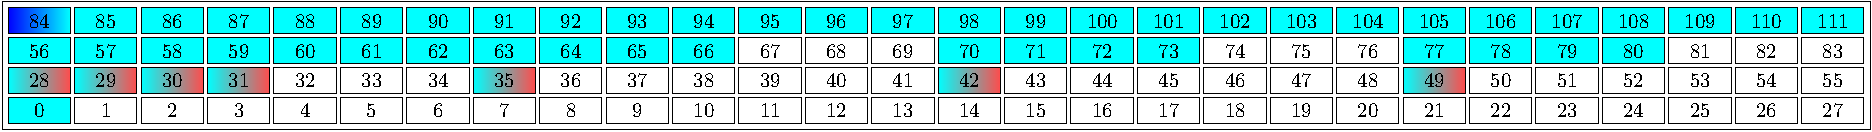
\includegraphics[width=\textwidth]{M-not-ED-m28.pdf}
	\end{center}
	\caption{Pictorial representation of the semigroup obtained with $m=28$. \label{fig:M-not-ED-m28}}
\end{figure} 
	\begin{figure}[h]
		\begin{center}
			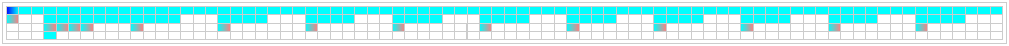
\includegraphics[width=\textwidth]{M-not-ED-m80.pdf}
		\end{center}
		\caption{Shape of the numerical semigroup obtained with $m=80$. \label{fig:M-not-ED-m80}}
	\end{figure} 	
\end{example}

Most of the indicated relations in the lattice represented in Figure~\ref{fig:lattice} have been treated along the text in this section. That  $\mathcal{D}$ and $\mathcal{M}$ are not comparable under quasi-generalization is shown in Proposition~\ref{prop:M-D-non-comparable}. Thus, the following has been proved:


\begin{proposition}\label{prop:not-chain}
	With the notation introduced, one has the lattice in Figure~\ref{fig:lattice}.
\end{proposition}
\thisfloatsetup{floatwidth=.35\hsize,capbesidewidth=sidefil,capposition=beside,capbesideposition=right}
%\thisfloatsetup[figure]{floatwidth=.35\hsize}
\begin{figure}[h]
	\centering
	\caption{Latice of some numerical semigroup properties (for quasi-generalization)}\label{fig:lattice}
	\begin{tikzpicture}[node distance=2.5cm]
	\node(S)        {$\mathcal{S}$};
	\node(W)  [below = 1cm of S]      {$\mathcal{W}$};
	\node(E)  [below right=1.5cm of W]     {$\mathcal{E}$};
	\node(M)  [below = 1cm of E]     {$\mathcal{M}$};
	\node(D)  [below of = W]        {$\mathcal{D}$};
	\node(D3)  [left of = D]        {$\mathcal{D}_3$};
	\node(G)   [below of = D]         {$\mathcal{G}_{60}$};
	
	\draw(S) -- node[left]{$\preccurlyeq$} node [right]{($=?$)}(W);
	\draw(W) -- node[left]{$\prec$}(D3);
	\draw(W) -- node[left]{$\prec$}(D);
	\draw(W) -- node[left]{$\prec$}(E);
	\draw(D3) -- node[left]{$\prec$}(G);
	\draw(D) -- node[left]{$\prec$}(G);
	\draw(E) -- node[left]{$\prec$}(M);
	\draw(M) -- node[left]{$\prec$}(G);
	\end{tikzpicture}
\end{figure}

Other comparisons could be made. As an example, fix a Wilf semigroup $S$ (possibly with small multiplicity when compared to the conductor). 
It is easy to check that $\multiplicityoper(D(S,a))=\multiplicityoper(S)+a$ and that $\conductoroper(D(S,a))=\conductoroper(S)+a$. Thus, $\frac{\multiplicityoper(D(S,a))}{\conductoroper(D(S,a))}= \frac{\multiplicityoper(S)+a}{\conductoroper(S)+a}$ tends to $1$ when $a$ tends to infinity. In particular, from a certain point on, the quotient $\frac{\multiplicityoper}{\conductoroper}$ is greater than $1/3$ and so, from that point on, all the semigroups satisfy $\mathcal{M}$. Therefore, $\mathcal{M}$ quasi generalizes the property corresponding to Proposition~\ref{prop:dilations}, for any fixed $S$.
\medskip
 
Denote by $\mathcal{P}_4$ the property associated to Proposition~\ref{prop:very-large-mult} with $\rho=4$.
As there are infinitely many semigroups satisfying $\mathcal{D}$ whose multiplicity is even, we get that $\mathcal{D}\nprec\mathcal{P}_4$. On the other hand, it is straightforward to check that there are infinitely many semigroups satisfying $\mathcal{P}_4$ and with small embedding dimension (less than $\multiplicityoper/3$). Thus $\mathcal{D}\nsucc\mathcal{P}_4$, and we conclude that $\mathcal{D}$ and $\mathcal{P}_4$, are not comparable under quasi generalization.
\medskip

Let $\embeddingdimensionoper\ge 10$ be an integer and denote by $\mathfrak{S}_{(\embeddingdimensionoper,\conductoroper)}$ the class of numerical semigroups with embedding dimension $\embeddingdimensionoper$ and conductor $\conductoroper$. Denote by $\ratiooper=\ratiooper(S)$ the ratio (second smallest primitive) of a numerical semigroup $S$. For fixed $\embeddingdimensionoper$ and $\conductoroper$, consider the set 
\[\mathfrak{R}_{(\embeddingdimensionoper,\conductoroper)}=\left\{S\in \mathfrak{S}_{(\embeddingdimensionoper,\conductoroper)}\mid \multiplicityoper \le \frac{8\embeddingdimensionoper^2}{25}+\frac{\embeddingdimensionoper}{5}-\frac{5}{4}\text{ and } \ratiooper >\left\lfloor\frac{\conductoroper+\multiplicityoper}{3}\right\rfloor\right\}.\]

Since no primitive of a numerical semigroup exceeds $\conductoroper+\multiplicityoper-1$, the ratio of a semigroup of embedding dimension $\embeddingdimensionoper$ must be at most  $\conductoroper+\multiplicityoper-\embeddingdimensionoper+1$.

Note that the class of numerical semigroups satisfying Equation~\ref{eq:prop-ratio} in Proposition~\ref{prop:ratio} is: \[\mathfrak{R}_{\embeddingdimensionoper}=\bigcup_{\conductoroper\ge\multiplicityoper}\mathfrak{R}_{(\embeddingdimensionoper,\conductoroper)}.\]

Consider now the class $\mathfrak{R}_{\embeddingdimensionoper}\setminus(\mathfrak{M}\cup \mathfrak{D})$. In set notation it may be written as follows:

\[\left\{S\in \mathfrak{S}\mid 3\embeddingdimensionoper < \multiplicityoper \le \frac{8}{25}\embeddingdimensionoper^2+\frac{1}{5}\embeddingdimensionoper-\frac{5}{4}, \conductoroper > 3\multiplicityoper \text{ and } \left\lfloor\frac{\conductoroper+\multiplicityoper}{3}\right\rfloor<\ratiooper \le \conductoroper+\multiplicityoper-\embeddingdimensionoper+1\right\}.\]
A natural question is whether this class is finite, that is, the disjunction of the properties $\mathcal{M}$ and $\mathcal{D}$ quasi generalizes the property associated to Proposition~\ref{prop:ratio} (with $\embeddingdimensionoper$ fixed).
Apparently there is no bound for the conductor, but a big conductor will force a big ratio. On the other hand, a small embedding dimension and a big ratio leads to a huge conductor. Is the starting ``conductor'' big enough?

% ===========================================
 
 
 
 
 
   

